\chapter{Analysis}
\label{cha:analysis}

This chapter focus on finding possible solutions to the problem described in our motivation with the lack of software engineers in the future. We will start by defining the quality \textit{availability} vs. our understanding of \textit{accessibility}. Thereafter we will focus on games, that are possible inspiration for the development of our final product. These games must both have a learning and entertainment aspect, and focusing on how some of the features that these game use can possibly be included in our game is an essential part of the analysis chapter. We will also shortly describe the theory behind gamification, and argue for what development tools/technologies we will use. We include a section about the interview with associate professor Kurt N{\o}rmark before making our problem statement and more clearly defining the requirements for our project and product.\newpage

%\input{tex/analysis/introduction}

%\section{Motivation}
\label{sec:motivation}

Many people interact daily with computers without knowing how a computer works.
There are many aspects of how a computer works, one being how programs are written.
Software is included in an increasing number of products, and it is a field that keeps expanding.\cite{idaArtikelMangel}\cite{forbesMoreProgrammers}
It is therefore important, that we get more people to realize, that computers are not too complicated and dangerous to work with.
We might be able to get more people interested in learning programming languages, if we provide a transition tool, that teach people basic programming constructs, and how these constructs can be combined to form working programs.
We define a transition tool as a stepping stone from one level of understanding of a subject to the next.\newline

Games are sometimes used as a learning tool, where the purpose is to have fun while learning.
However, in our experience many edutainment games (entertaining educational games) do not engage students sufficiently into learning and few exist that focus on older children and young adults. 
We are therefore motivated to create an engaging edutainment game as the transition tool, where the target consumers are anyone who wants to learn basic programming skills and do not have a higher degree of understanding of mathematics. This is relevant for the paradigm, that we choose to focus on, which is the imperative paradigm. See \autoref{sec:interview} for a discussion of what paradigm to focus on.\newline

With the introduction of tablets and applications, the market for games has increased, and many edutainment games are available on these platforms; iOS, Android, and Windows phone.
It is important for us, that the product developed during this project has the potential be used on many platforms.
The motivation for creating a highly available product is to provide many people with a transition tool in the form of a web application, that makes basic programming skills more attainable.\newline

It is important to state, that the motivation is not to teach users a specific programming language.
Rather it is important for us, that constructs in mostly imperative languages are understood, such as if-else-statements, for-loops, variable types and handling of variables, and that the user can get a visual representation of when a program is executed. We have chosen to focus on constructs in the imperative paradigm, since it is the first paradigm software engineering and computer science students of Aalborg University are introduced to and based on our interview with Kurt N{\o}rmark, see \autoref{sec:interview}.\newline

Essentially the motivation for developing an exciting and engaging edutainment game in this project is to make people interested in programming by providing a transition tool and having them consider getting an education in Software Engineering, so that the increasing demand on software in the future can be met by the number of educated software engineers.\citep{idaArtikelMangel}
%\section{Software Engineering Method}
\label{sec:software_engineering_method}
This section will shortly describe the software engineering method used during this project, how it was chosen and how we intend to implement it into our project.

\subsection{Choosing a Development Method}
There exist many different development methods, such as Scrum, \ac{xp}, \ac{up}, and the classic waterfall method.
This project rely heavily on initial analysis before starting to design and implement, since the problem was not clearly defined from the beginning.
Using \ac{xp} to instantly write code would therefore not be suitable for this project, and for that reason, it was quickly discarded.
Scrum is suitable to implement in projects where requirements to the final project often change.
It includes cycles, called sprints, that include analysis, design, implementation and testing.
We did not feel, that Scrum was suitable for our project, since the requirements, when determined, are fairly static.
The static nature of the requirements might make it possible to implement the classical waterfall method, but given our prior knowledge from lectures, the waterfall method is generally not very usable and potentially limiting by having to declare on part of the process finished before starting the next.
Therefore, we decided to use \ac{up} as the development method.
\ac{up} divides the software development processes into the following four phases: 

\begin{itemize}
\item[Inception] The project's boundaries and scope should be defined, as well as risk identification and preliminary project schedule.
\item[Elaboration] The team is expected to create the majority of the system requirements and establish the system architecture.
\item[Construction] This should be the largest phase in the project, since this is where the system is implemented.
\item[Transition] The project is deployed and feedback is incorporated into future releases.
\end{itemize}

Each phase is divided into iterations and will contain most of the activities associated with software development (analysis, design, implementation and testing), but to varying degrees. As can be seen in\autoref{fig:up}, the main focus will gradually shift from one activity to the next in the process.\todo{Barbara: Source of picture please}

\begin{figure}[ht]
  \centering
    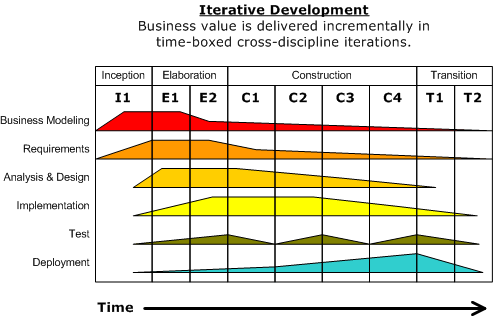
\includegraphics[width=\textwidth]{img/Development-iterative.png}
  \caption{Phases and activities in UP}
  \label{fig:up}
\end{figure}

%Given that this project is estimated to require a long time spent on analysis before actual development can take place, an iterative method with short cycles spent on all activities, such as SCRUM, would not be suitable for this project. XP as a possible development method can also be discarded for the same reason.\newline
%Instead the group will begin by focusing on the analysis, definition and scope of the problem to be solved. It will then move on to design of the solution along with prototype implementation and testing of these. Finally the product will be tested and findings during the testing will be implemented. 

The fact that \ac{up} is divided into phases that each have iterations fits well with the group's wish to focus mostly on one development activity at a time, without using the dated classical waterfall structure of the project.
\ac{up} also initially focuses on requirements and analysis, which is suitable for this project.\newline

Now we will describe how we intend to implement \ac{up} into our project.

\subsection{Implementing UP}


\subsubsection{Inception}


\subsubsection{Elaboration}


\subsubsection{Construction}


\subsubsection{Transition}


\section{Availability}
\label{sec:availability}
Before analyzing possible products, that can be used as inspiration for the project, the concept of availability is introduced. Availability is not the most essential part of our project, however the concept is used later in the report to describe useful properties of products. That is the reason we start by defining our understanding of the term.\\ 

In computer science, availability is defined by the up time of a software product, meaning how often the product can be used.\cite{defAvailability}
In this report, we define good availability as the ability to easily obtain and use a piece of software.
It should also be noted, that we distinguish availability from accessibility, where accessibility is more focused on how easy a piece of software is to use for people with disabilities.
Accessibility is not a focus in this project and will not be discussed in further detail.\newline

The availability of games is a concern, when dealing with edutainment games.
Some games are only available in public schools, providing a license to a bundle of games, while others are sold commercially.
This limits the time a user can actively interact with the game and in the case of edutainment games, it will also limit the learning potential.
Commercial games have a higher degree of availability, since they are sold in stores which means a single license can be bought by anyone.\newline

With the widespread introduction of portable devices, such as tablets and smartphones, many games are now available on the go.
This serves a useful purpose, since children can interact with the games, for example on long trips or during other long periods of inactivity.
This also increases the availability of games.
Many game applications are miniature games, that are sold at a low price, around $\$0,99 (6,00 DKK)$.
The low price increases availability.
Also, given that many of the newest portable devices support fast mobile Internet (3G and 4G), it is possible for users to access the Internet everywhere.
Making a web based edutainment game is therefore mostly restricted by the availability of the Internet, be it either wifi or mobile.\newline

To achieve a high degree of availability, it is intuitive to make products for a widely used platform, the initial cost of entry should be low or directly reflect the quality of the product, and it has to have a high degree of visibility.
We define visibility as the ability of a product to be easily found by the customer.
Methods to increase visibility include, but are not limited to, advertisement and active use of social networks.
\section{Edutainment in Schools}
\label{sec:eduinsch}
The popularity of edutainment in Danish schools has increased in recent years, from being seldom used to a more commonly used tool for learning. 
This can primarily be observed by the release of various web portals \footnote{Websites that serve as a gateway or a main entry point on the Internet to a specific field-of-interest or an industry.\url{http://www.businessdictionary.com/definition/portal.html}} for teachers to find edutainment oriented games and the recent purchases of iPads and other tablets or similar electronic devices for use both in schools and at home for homework.
This change in opinion about edutainment resources is rather interesting. For that reason, this section will describe what kind of tools schools use as part of their edutainment catalogue for teaching and provide an overview of what a good and useful game for a school is.


\subsection{Games in Schools}

The games currently used in schools are typically miniature, obscure titles, that are not well known outside of the school environment.
In other words, there are few edutainment titles, that have made a breakthrough in commercial terms.
A few of the most commercially well known titles are 'Global Conflicts: Palestine', the 'Magnus og Myggen' (Magnus and the Mosquito) and 'Pixeline' series.
We have chosen to focus on 'Global Conflicts: Palestine', because it is targeted at older children, which will be the primary focus group for our final product.

\subsection{Properties of Edutainment}

Edutainment is still debated as a term. Mitchel Resnick of MIT Media Laboratory dislikes it because we teach children from a young age that education is a passive activity, a service provided to you. And one that is boring and should be livened up with entertainment - another word he claims has passive, service-oriented connotations. Instead he prefers the term "playful learning", because playing and learning are activities that focus on the process instead of being means to an end. The key to successful playful learning, he says, is to use the child's intrinsic motivation and curiosity around a subject to help them learn about it. The challenge, he says, is that many people today view games and play as not having any value when it comes to teaching people anything. 

In Mitchel Resnick's definition, what this project should achieve is playful learning, however it will continue to be called edutainment, due to the fact that his definition of playful learning is the same as the group's definition of edutainment. The properties of edutainment should be that it is

\begin{itemize}
\item Intrinsically motivated, i.e. the child should want to do the activity, not have an external source of motivation for it such as a teacher saying they must do it.
\item Focus on the creative process of trial and error without necessarily having any scientific approach or pre-existing hypothesis to test.
\item Give the child hands-on experience with the subject matter (e.g. mathematics or physics).
\end{itemize}\cite{edunoty}

While the target audience in this project  may not be children, the properties listed above can also apply to older people, as curiosity and creativity are traits that do not disappear with age.

\subsubsection{Global Conflicts: Palestine}

Global Conflicts: Palestine was created by a small Danish company called 'Serious Games Interactive' in close collaboration with Copenhagen's IT University.
The purpose of the game is to teach children about the highly complex conflict between Israel and Palestine.
In the game, the player is a reporter, who has to report on the war.
While playing, the player will create articles, include pictures, and make headlines, that will shape the opinion of the newspaper's readers.
The game includes a basic communication system, where the player chooses between different dialogue options to gain trust and uncover the true story behind the conflict. 
\begin{quote}
	In general, Global Conflicts: Palestine proved to be a very successful and powerful alternative to the traditional primary use of books in Danish schools.\cite{laeringpaaspil}
\end{quote}
The game, when bought with a school license, is sold in a bundle, that includes the game and a task sheet for the students.
The task sheet asks the students to answer questions and solve puzzles relevant to the game, right after playing.
Furthermore, it is possible for the teacher to monitor the students as they play through the game, via a separate computer using the same network as the players.
This feature allows the teacher to pin point when a student is having difficulties with a task, or when an opportunity to further increase the student's learning experience arises.\newline

In many ways 'Global Conflicts: Palestine' is a game, that has reshaped the opinion about edutainment in schools. It has been able to keep the teacher in the center role in the students' playing experience, by ensuring that the student is focused, and playing the game becomes a learning experience.\cite{laeringpaaspil}\newline

The title is praised for the way that it combines learning and playing.
The game is about a real conflict, which makes it more engaging.
It forces the player to make important decisions, that can have consequences later in the game which also makes it engaging.

\subsubsection{Tablet Games}

Some schools already use games, that teaches the student about grammar, spelling, mathematics, etc., and some of these games have started emerging on mobile platforms as well.
Typically sold as commercial games (i.e not school licensed), they are available to everyone for a small fee or in some situations mainly paid for by advertisements.
Two examples of these games are 'Trunky Learns Numbers' and 'Trunky Learns Words', which are games created by the company 'Serious Games Interactive'.
These games are available to the children in Odder Kommune in Denmark, and are used to further enhance a student's learning experience.\cite{odderipad}
The appearance of these games on the tablet market suggests that edutainment games do not necessarily have to be large and complex like 'Global Conflicts'.
Unfortunately, due the very recent agreement to go through with the plans of bringing iPads into schools, it is too early to have enough valid data to document any positive change in the learning experience of the students using tablets actively in their education.
However, the research and personnel group have noticed an increase in motivation, knowledge sharing, social competence and acceptance, as well as a focus on education that engages the students and a focus on delivering useful results amongst the students.\cite{odderipadpjece}
In this example the tablets are used for more than playing various games. They are also used to creatively engage the students, coordinate learning, and do other IT oriented projects.\cite{odderipadpjece}
\section{Edutainment for Private Consumers}
\label{sec:privateconsumers}
Many companies create educational games for children to learn mathematics, languages and other basic school topics.
Most of these games are targeted towards younger children, who are either about to start school or in elementary school.
A company like Krea Games creates multiple series for children of various ages.\cite{kreagames}
These games are mostly available for PC, with a small subset also being available for Android and iOS devices.
In this section, we will examine some of the best selling educational games for private consumers.

\subsection{Best Selling Edutainment Games}
One of the most popular edutainment games is 'The Oregon Trail' with more than 65 million copies sold worldwide since its initial release in 1982.\cite{oregontrail}
The game was originally released to teach children in American schools about how pioneers lived in the $19^{th}$ century, but was also released to the general public as a standalone game for the PC. 'The Oregon Trail' was one of the first video games ever used in the United States for educational purposes, which has added significantly to its popularity.

The objective of the game is to help a group of American pioneers follow the Oregon trail and make sure, that they survive their endeavor to finally settle down in Oregon. The game teaches children the history of the Oregon Trail without sacrificing the gameplay experience and thus the game is considered a good game even without the educational aspect.\newline

As with 'Global Conflict', the game includes a sense of realism.
Random events play a large role in Oregon Trail.
It is possible to die from various diseases (such as dysentery), cattle being stolen, food rations getting low etc.
It seems, that focusing on making the game feel more realistic to the player is part of the engaging nature of both games.
Neither of the games impress in terms of graphics however both games do possess a sense of realism. From this it can be extrapolated that it is less important how the game looks graphically and more important to focus on creating a realistic situation, that the players want to interact with and learn more about.\newline

Other popular edutainment games include:
\begin{itemize}
\item "Where in the World Is Carmen Sandiego?", which is a game released in 1985, that teaches geography.
The game was popular enough to spawn several sequels released as late as in 1998 and the first version of the game was released in 2011 as a Facebook game.\cite{carmensandiego}
The game is centered around the detective Carmen, who travels around the world in order to capture criminals.
Learning geography is an essential part of the game, since the player has to follow clues to where in the world a thief, she needs to catch, has gone. Later games in the series taught different subjects such as history or mathematics. In order to become a better player the user has to improve their knowledge of the topics in the game, which is extremely useful and shows that the process of learning while having fun is definitely possible and attainable in video games.

\item "Lemonade Stand" is a game created by Bob Jamison and released in 1973, which teaches the player about economics.\cite{lemonadestand}
It is a game, where the players play as a child who has a lemonade stand.
The player makes choices regarding the cost of the lemonade, money spent on advertising, and how many glasses of lemonade to make, thereby teaching basic economics in a fun way, that children in some cultures can relate to.
The everyday situation of the game makes it very relatable. 
Even though lemonade stands are not a common sight in Denmark, the aspect of making the game, so that the user can relate to the situation, seems to be an important factor.
Maybe this is one of the aspects that have made the game popular enough that several remakes of the game has been released throughout the years.
\end{itemize}

By analyzing and comparing these games, it is possible to create a game that is both engaging and educational, while avoiding making it too obvious that the game is trying to teach the player something.
Thus the player does not feel like they are doing homework while playing the game.
We have seen, that the aspects of realism in 'Global Conflicts' and making the game relatable in 'Lemonade Stand' may be part of the reason for the success of these games, and that, if possible, these aspects should be included in our game.

\subsection{Browser-based Edutainment Games}
Most edutainment games, that can be accessed from a browser on the PC are flash games on websites.
Some of these claim to be approved by teachers for educational purposes.
Many of the games that we have found are heavily inspired by classic games, such as a Pac-Man like game called Math Man, where the player has to play Pac-Man while doing math problems to win.\cite{mathman}
Grand Prix Multiplication is another example, which is a multiplayer racing game, where the player has to do multiplication to make the car drive faster in order to win.\cite{grandprix}\newline

Browser-based games are good in terms of availability, since most households have a PC and in many cases, each family members has their own device with access to the Internet. Most browser-based games are free-to-play, which increases their availability. However, our overall impression of the browser-based edutainment games is, that they are very explicit in their teaching method. This can be a good thing if the game is primarily used in schools, where the purpose is to teach new material. However, the explicit teaching nature of these games can make them seem like homework and keep the children from playing the games in their spare time. We found, that in general the games we look at neglected the entertainment and engaging aspect of video games. It is important to avoid explicit teaching in our final product.
\section{Teaching Programming with Games}
\label{sec:teachProgWithGames}
We have not been able to find many games, that try to teach programming fundamentals. 'Carnage Heart' for the original PlayStation is one of the few, that exist. In the game, the player has to create a robot, that has to fight other robots in a war. However, the robot cannot be controlled directly, instead the player has to program its behavior using a grid of icons, as seen on \autoref{fig:carnageheartsoftware}.

\begin{figure}[ht]
  \centering
    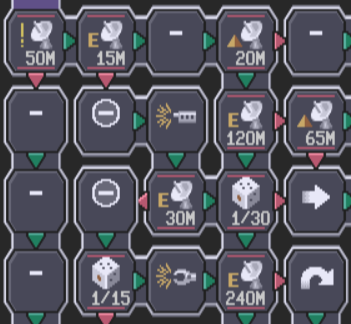
\includegraphics[width=0.5\textwidth]{img/CarnageHeartSoftware.png}
  \caption{Screenshot of the programming interface in Carnage Heart.\cite{carnageheartsoftware}}
  \label{fig:carnageheartsoftware}
\end{figure}

'Carnage Heart' teaches basic programming constructs, but it does not present them as such. Instead the player is presented with a set of rules, which are much like the rules of programming, and are told to create what is basically an AI for the robot.\newline

Another example of a game trying to teach programming is 'CodeCombat'. \cite{codecombat} 'CodeCombat' is a browser-based game, that tries to teach JavaScript programming by making the player write code to play an RPG. The player plays as a wizard, and the programming is represented as magic spells in the game. The player is programming an AI for a knight, that has to fight a variety of monsters. Control of the knight includes movement and attack as well as conditions such as attack if the enemy is in range.
Although 'CodeCombat' is a game, it is very explicit in its teaching, because the player has to write the code and not just drag objects around on the screen. Tools such as 'Codecademy' provide the same kind of programming guides as 'CodeCombat', but without the gaming aspect.\cite{codecademy}\newline

Microsoft has released a game for teaching children programming called 'Kodu Game Lab'.\cite{kodu}
'Kodu Game Lab' is a free game on the PC and can be bought for $\$4.99$ on the Xbox360 marketplace.
This means, that the game is available to most possible users.
In the game, the player starts with a small world, which is a square of grass.
The player can then add objects and program them to do what the player wants.
It is possible to make an object react to other objects, e.g. eat them if the object is above the another object.
The programming interface for 'Kodu Game Lab' shown on \autoref{fig:kodu} is structured in a input/react way, that visually illustrates what will happen when some condition is met. This is is basic principal of if-statements, but the game does not include constructs such as loops or variable declaration, which will be a part of our final product. However, the simple drag-and-drop and click approach to programming avoids the need for the user to write code, thereby limiting how explicit the learning process is in the game.

\begin{figure}[ht]
  \centering
    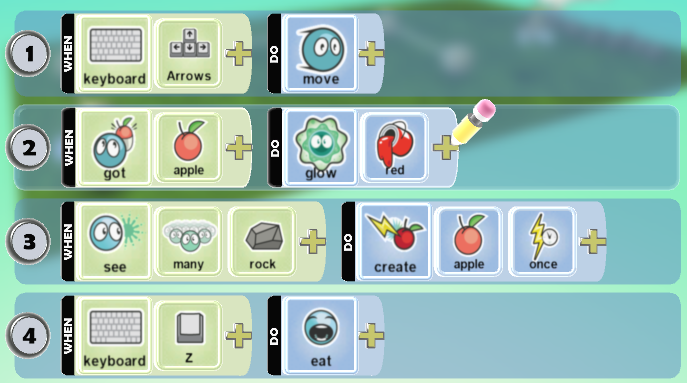
\includegraphics[width=\textwidth]{img/kodu.png}
  \caption{Screenshot of the programming interface in Kodu Game Lab.}
  \label{fig:kodu}
\end{figure}

The way 'Carnage Heart' and 'Kodu Game Lab' approach teaching basic programming constructs is relevant to our project, since they approach similar approaches to teaches basic programming constructs and could therefore be a source of inspiration in the design phase of this project.\todo{From Martin: If you will have time try to be more specific how these games are relevant for your project.}
\section{Gamification}\label{sec:gamification}
\todo{Maybe make it more clear what problem gamification attacks? Section explain gamification really good, but I miss some a little more analysis.}Gamification is "the process of game-thinking and game mechanics to engage users and solve problems" \cite{Zichermann2011}, i.e. using core elements of games to attract users and keep them coming back to a specific task.

Gamification is used in many areas, for example in engaging users in solving complex tasks: The game FoldIt, developed by University of Washington in 2008, employs people in folding proteins, which is a job that the brute-force approach of computers does poorly compared to man's natural abilities with regards to spatial reasoning and 3D pattern matching. In 2011 a team of users managed to decode an AIDS-causing monkey virus in just 10 days, a task which had been unsuccessfully attempted by scientists for 15 years.\cite{Huff2011} Today, the game has almost 500.000 registered users, using their spare time folding proteins for science for free.\cite{FoldIt2013}

FoldIt works, because it employs game mechanics and dynamics that correlate quite well with primary human desires to keep people interested and engaged in the activity.
Figure \ref{fig:bunchball} shows the interaction between human desires such as status, competition and rewards.

\begin{figure}[hptb]
  \centering
    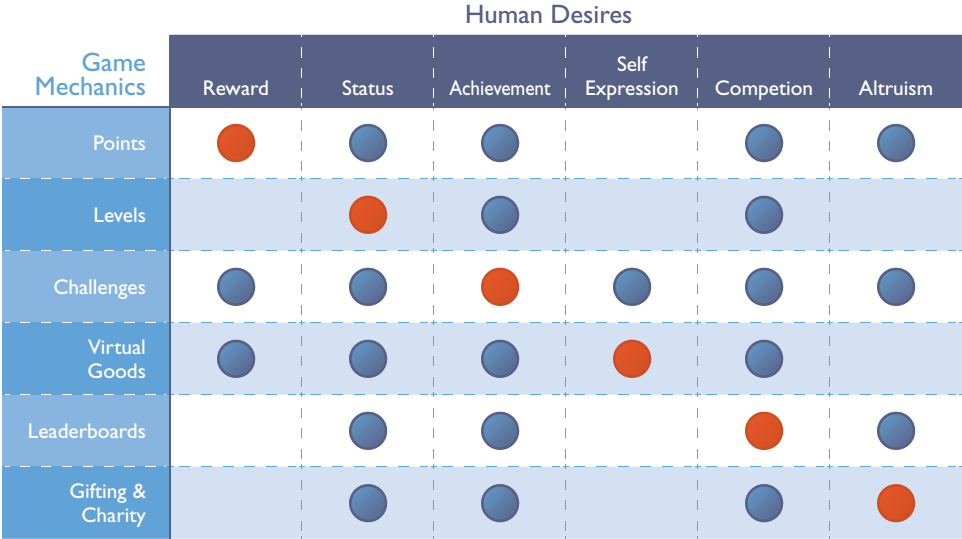
\includegraphics[width=\textwidth]{img/bunchball.png}
  \caption{Interaction between Human desires and Game mechanics}
  \label{fig:bunchball}
\end{figure}

\todo{Really good analysis part of the section}As can be seen, the human desires can be fulfilled via various game mechanics. In FoldIt, for example, a Leaderboard allows the users to compete against each other either as groups or soloists, which allows both individualists and team players to participate with a feeling of fulfillment. 

If these game mechanics are used, many people will feel entertained while using the product. This is beneficial to a product that, for example, educates the user. In the online application FreeRice, developed for the World Food Program, the user's desire for altruism is fulfilled via donations of rice grains for completed tasks, while general academic skills are honed, such as vocabulary and basic mathematical proficiency. Again it is possible to join groups, and there is a leaderboard, thereby introducing an element of competition.\cite{freerice}

As has been described, the game mechanics in Figure \ref{fig:bunchball} will give people an extrinsic motivation (rewards, leaderboards etc) to keep playing, although the activity might not carry any intrinsic motivation for the user. This is useful in education, because people tend to easily give up, or simply never really start, when acquiring knowledge and skills that, while useful, may not be their primary field of interest. Keeping people entertained while learning can ensure that they spend more time on the subject and may also pique their interest in an area they might not have explored by themselves.
\section{Web Development Technologies}
\label{sec:tools}
When developing a browser-based game, several different technologies are available.
Six of these are of some interest; HTML5, Flash, Java, Silverlight and Unity, since they provide easy development of internet graphics, games and animations.
They are also some of the most well known web development technologies.
The reason that these specific technologies are so widely used is, that each has had a large focus on applications embedded in browsers, either natively, as is the case of HTML5, or through plug-ins.
The development tools for Flash are, however, not free, and as such not an option for this project.\cite{adobe13}
Besides, Flash has been discontinued from mobile platforms,\cite{adobe12} and would limit the availability of the game, which is an important consideration, see \autoref{sec:availability}.
The rest of the tools will be introduced in this section, mostly focusing on the portability of each tool, as measuring differences in performance and prevalence of required plug-ins and the like is virtually impossible.
Another focus, given the scope of the project, is that the game should exist solely as a web application, and not a standalone game, app or similar.

\subsection{HTML5, Canvas and WebGL}
HTML5 is the latest standard for implementing web-pages, and the current recommendation from \ac{w3c}.\cite{html513}
It includes several useful APIs for implementing multimedia, specifically the canvas element, which provides an area, where graphics can be drawn.
HTML5 games will be written in \texttt{JavaScript}, which is interpreted by the browser, and as such is available on most computer systems.\todo{From Martin: I know that its very unlikely, but what happens when JavaScript is disabled?}\newline

The canvas is an element in the html that allows us to draw or import pictures, also known as sprites.\todo{Jeppe: Is this a correct understanding of the canvas element? Otherwise is there a better description and can we reference forward to our implementation section?}
The canvas can be further improved using the WebGL extension, which allows for hardware accelerated graphics in the canvas.\cite{khronos13}
This will eliminate much of the low performance, that can arise from software accelerated graphics.
Additionally, WebGL is implemented by default in all modern browsers, including some mobile browsers, so most users will be able to play the game without downloading any additional software.

The main disadvantage of a HTML5-based solution is, that it is a relatively new technology, and for that reason problems could occur, where an optimal solution has yet to be found, which could increase development time.
Various browsers support HTML5 differently.\todo{Could you be a bit more specific which browsers do not support HTML5? Maybe we could visit html5test.com on various devices and compare result?}

\subsection{Java}
With Java it is possible to create applets that run in a browser.\cite{java13}
These applets can be used for any type of applications, including games.
The greatest advantages of using Java for applets is its large user base and library collection, which means that a lot of the technical difficulties in building a game has been solved by other people, and open source solutions are publicly available.\newline

The disadvantages of Java is, that it is an external browser extension, and it is not installed as a standard on most systems.
This means that the user might have to install and keep the extension updated themselves to use the game. 
This could also be an annoyance for institutions having to keep several computers up to date, especially since Java is updated quite frequently, often close to $10$ times each year.\cite{javahistory13}
Additionally, to get it to work on Android systems, it needs to be in the app store, and for iOS systems, Java support is limited in general.

\subsection{Silverlight}
Silverlight is very similar to Java applets, but developed by Microsoft and typically programmed in either C\# or Visual Basic.\cite{silverlight13}
Though Silverlight has historically had a focus on media streaming, today it is a multipurpose framework and most of the same advantages and disadvantages as Java had also apply to Silverlight.
A choice between Silverlight and Java is therefore mostly based on personal preference on the side of the developers.

\subsection{Unity}
Unity is a game development framework, capable of publishing games to browsers.\cite{unity13} 
While Unity is focused mainly on developing 3D games, there is support for any type of game.
Using Unity would provide a useful framework for game development, but distribution could be problematic.
While Unity games can be ported to virtually any OS, desktop or mobile, the browser plug-in is only available for Windows and MacOS.
For the rest of the platforms, the game has to be released as a standalone application, which goes against the goal of creating an available web application.

\subsection{Summary}

An overview of the compatibility of each technology described on various platforms can be seen in \autoref{fig:technologies}

\begin{figure}[ht]

\begin{tabular}{|r|l|l|l|l|l|}
\hline
 & Windows & Linux & MacOS & Android & iOS \\
\hline
HTML5 & Full & Full & Full & Partial & Partial \\
\hline
Java & Plugin & Plugin & Plugin & Standalone only & Limited \\
\hline
Silverlight & Plugin & Plugin & Plugin & Plugin & None \\
\hline
Unity & Plugin & Standalone only & Plugin & Standalone only & Standalone only \\
\hline
\end{tabular}
\label{fig:technologies}
\caption{Technology compatibility overview}
\end{figure}

All of these technologies are capable of very similar functionality and portability.
This means, that the decision was mainly based on how easy it is to distribute, as well as personal preference of the developers.
In the end, HTML5 and WebGL was the chosen platform.\todo{maybe quickly list of why it has chosen. Or just say that based on the sections above, we evaluate HTML5 and WebGL to be the best option.}
\section{Interview}
\label{sec:interview}

To found the basis for the requirements it was necessary to conduct an interview with someone knowledgeable in the field of teaching programming to 
students. For that reason, it seemed obvious to set up an interview with the associate professor Kurt N{\o}rmark at the institute. There are many 
different ways this interview could have been set-up, but the group decided to take a semi-structured approach simply based on good experiences from 
past interviews. 


The semi-structured approach allows us to conduct the interview in a less strict way, which in our experience works better when the goal of the 
interview is to achieve knowledge and learn-as-we-talk, as opposed to holding the interviewee to certain facts as seen by journalists in media. The 
interview was conducted by two group members, who had created a list of \textbf{must-answer} questions to help guide and create focus points for the 
conversation and drive the interview toward a goal. The interview could then be considered successful, once all of these questions had been answered - 
the details and information given between these questions is then bonus knowledge, that we would not have otherwise achieved, if the interview was a 
strict, and fully structured interview.

One of the participants at the interview was responsible for writing down the interviewee's answers, and participated only somewhat in keeping the 
conversation going, whereas the other interviewer was responsible for keeping the conversation going entirely and asking new questions, when necessary. 
The main questions that were posed during the interview are:

\begin{itemize}
	\item Which advantages are there teaching students how to program in the Imperative Paradigm first, and not in a different paradigm?
	\item Which disadvantages are there?
	\item What is the biggest difficulty for new students when they are introduced to imperative programming?
	\item Which programming constructs / types are the most difficult for students to understand (in the imperative paradigm)?
	\item What would you like the students to be better at, when they begin the Imperative Programming course?
\end{itemize}


\subsection{Results of the Interview}

The following will go through the main points of interest for each of the questions that were asked. Notice that the questions below has been slightly 
reformulated to better fit the knowledge that was given throughout the interview. They correspond to the questions in the previous section, but 
information has been added, as was given during the interview.

\subsubsection{Why is the Imperative Paradigm taught first, and not a different paradigm?}

Starting with the \textbf{Object-Oriented Paradigm} seemed counter intuitive, because it would teach the students how to classify their code, but not 
write their code. One of the main points that were brought across for this question was that it was important in the beginning that the student 
understood how to write code, before they started to worry about classification of this code and storing it in classes. In other words, it is important 
that the student understands \textbf{what} to structure \textbf{before} he/she structures, and this can not necessarily be taught to new students by 
starting off with the \textbf{Object-Oriented Paradigm} or rather - perhaps it could, but it would be more efficient to teach by using a different 
paradigm first. 


As for not using the \textbf{Functional Paradigm}, Kurt N{\o}rmark actually believes that starting with the functional paradigm is the most sensible 
way of teaching programming to new students, because it is very mathematically inspired, the level of abstraction is much higher, and so it would be 
easier for a student to simply see the code they write in a more mathematical way. In other words, the \textbf{Functional Paradigm} would be ideal for 
students, who has completed \textbf{Math A}, which would teach students how to call functions with functions (think integral and differential equations)
 - Math A is a prerequisite for the \textbf{Software Engineering} and \textbf{Computer Science} education at Aalborg University.\todo{Source on 
prerequisite}


For students who has not yet completed \textbf{Math A} or may have, but are not comfortable with mathematics, starting in the Imperative Paradigm would 
arguably be a much better decision. The basic philosophy behind the imperative paradigm is 'first-do-this and next-to-that'. This philosophy is known 
to many as a listed structure like in manuals or recipes, which is also an argument for starting with the imperative paradigm.


\subsubsection{What is the biggest difficulty for new students that are introduced to imperative programming?}

There are many parts to the problem for a new student who has to learn how to program from scratch. However, a recurring theme is the level of 
abstraction. It can be quite a mouthful for some new students to understand a low level language, which often is used for the Imperative Paradigm, - 
think C. Things that execute sequentially are generally not so difficult to understand, but it can be very difficult to understand the low level 
mechanics of the computer, and how the language interacts with the machine. This leads to the conclusion that the lower the level of abstraction, the 
more difficult it is to understand for new students.

\subsubsection{Which programming constructs / types are the most difficult for students to understand (in the imperative paradigm)?}

It is not so much a problem with the constructs - \textbf{for's} and \textbf{while's} are generally simple to understand for the students, but implicit 
constructs like recursion can be a bit of a mouthful, and even so for more experienced programmers who has completed several semesters in the 
education. As for types, understanding that a Boolean type is as valid a type as an int or a char, can be difficult for the students - computing more 
complex, or large boolean expressions can cloud the execution of a students program extensively, and make them lose track in the flow of their program, 
which leads to errors and confusion. Using operators such as bit shifting can also be tricky for the students, which is a result of the very low level 
of abstraction this yields for the students, which backs up the point noticed previously; the lower the level of abstraction, the more difficult it is 
to understand - the higher the level of abstraction, the easier it is to understand.


\subsection{Conclusion}

The interview yielded useful results for the project, and taught us what aspects of programming are more difficult for a new programmer to wrap 
their mind around. The above findings will be summarized in the below paragraphs.

\subsubsection{Constructs}

One of the key findings of the interview was the discussion on \textbf{level of abstraction} and how it was relevant for constructs. As a rule of 
thumb, Kurt N{\o}rmark explained that the level of abstraction should reflect the constructs used within the program. Consider the following example, a 
higher level language such as Java makes use of a \textbf{for-each} construct which allows the programmer to iterate through the elements in a list 
easily - on a single line of code in fact. A C equivalent could be a \textbf{for} construct, which would iterate through an array, with explicitly 
stated variables that are incremented at each pass through the loop. By the way the \textbf{for} constructs has been implemented in the two languages 
it is easy to see that C has a much lower level of abstraction, than Java does, because you do not explicitly declare conditionals or variables. 
However, the C-like \textbf{for} construct has also been implemented in Java (it uses both kinds). 

\subsubsection{Target Group}

Determining the paradigm of our program will largely depend on the target group for the software. It turns out that if students are mathematically 
educated - or rather, students have completed up to \textbf{Math A}, it would be better to let the software follow the Functional Paradigm, because 
they could better relate to our software this way - they have seen it before, basically. Otherwise it would be far better to start with the Imperative 
Paradigm. This could also be the case if the students are generally not very strong mathematically though they have completed \textbf{Math A}.

\subsubsection{Sequential Execution}

The reason Boolean types in languages can prove to be a bit of a mouthful for a new programmer to understand is that they can obfuscate the trace of 
execution through the program. The simpler the execution of the program, the easier it is to grasp for the student. It may be obvious that the 
Sequential Execution is the most simple form of execution there is, but if the software includes boolean types, it is not always possible to deduce 
what is the next bit of code which will run. Therefore to make the program simple to understand and read, sequential execution would work best, with a 
bare minimum of boolean types, which incidentally is the hardest type to understand.

\subsubsection{Level of Abstraction}

The lower the level of abstraction the more does the programmer need to know about the computer which runs the software. Therefore, for teaching 
purposes a higher level of abstraction is considered easier for students to learn than a language with a low level of abstraction.\todo{return later}
\section{Problem statement}
\label{sec:problemstatement}

Today's world has a great need for programmers. Jobs for Software Developers are some of the best ranked in studies of the most well-paying, secure jobs to get. This is because there is a need for these people, and the need will only continue to grow as more devices become smarter and need software to run them.
Many people find computers and especially programming daunting, even though they might be good at it if they knew more about it.\newline

\begin{quotation}
	How can an edutainment game be designed as a transition tool, to give people a taste of basic programming constructs, without \todo{Maybe to subjective:} making it obvious and scaring them away before they know what it is. How can gamification techniques be utilized to make the game entertaining and engaging for children over \todo{age} to learn how to program or teach them constructs in the imperative paradigm?
\end{quotation}

\section{Requirements}
\label{sec:requirements}

The requirements for this project are divided into practical (game-related) requirements and requirements with regards to the edutainment-oriented 
aspects of the project. First the edutainment requirements gathered from the analysis will be presented, followed by the game-related requirements.

\subsection{Edutainment}

From the games examined in \autoref{sec:privateconsumers}, \autoref{sec:eduinsch} and \autoref{sec:interview}, the following requirements have been 
established: 

\begin{itemize}
	\item The Global Conflict and Where in the World Is Carmen Sandiego? series focuses on being helpful for different subjects such as social studies 		
	and medialogy. While this is commendable, it is out of scope for this project. This project should focus on teaching a single subject.
	
	\item The graphics of Global Conflicts are mediocre compared to games put out by commercial game studios. However, Global Conflicts is a popular game 
	despite the lack of good graphics. This showed us that there does not necessarily have to be a relation between the level of graphical detail in 
	games, and the game's potential popularity. For this reason our game will be a 2D game.
	
	\item Many tablet games are targeted younger children and as such, considerations for a more mature audience should be made.\todo{Anders: Hvad mener 
	vi om dette requirement? jeg synes det skal slettes.}

	\item The Oregon Trail manages to make learning engaging without sacrificing gameplay by depicting a realistic situation, that the player can 
	interact with. This type of relatable gameplay should be included in the game as well.

	\item The browser-based games in general are very explicit in their intend to teach. It is a requirement, that our game avoids this issue, 
	since our idea is to teach people basic programming constructs without explicitly stating "now you are learning!". 
	
	\item The game must take care in how the level of abstraction is represented because the game is intended to teach programming. The level of 	
	qualification the players have at the start is considered basic at best, therefore a higher level of abstraction is necessary to succesfully teach.
	
	\item When the user interacts with the program it is important that they write code that runs sequentially, such that the flow is predictable. This 
	ensures that the program they write is easier to understand, but the program editor as well works in a predictable way.
\end{itemize}

\subsection*{Practical}
\begin{tabular}{|l|l|l|}
\hline
\multicolumn{3}{|c|}{Requirements}\\
\hline
Need & Want & Nice\\
\hline
Graphics & Save/Load & Animation\\
Program Editor & Multiplayer & Leaderboards (Ranking system)\\
Environment & Challenges & Tutorial (Interactive)\\
Manual & AI & Export/Import\\
 & GUI/HUD & \\
\hline
\end{tabular}

The reasoning behind the priorities are as follows:
\begin{itemize}
\item Graphics are highly needed, because the game emphasizes a visual approach to learning programming constructs and a console oriented approach 
would therefore not be viable.

\item A Program Editor is needed to allow the users to interact with the game.

\item Environment covers the world in which the user's code is executed. This is the "playing field" of the game, where the user sees the results of 
their programming and as such is essential to make the game engaging.

\item A Manual is needed to teach users how to interact with the game. Optimally, the game should be designed to naturally teach the player how to play 
the game without a manual, but in the case that this is not achieved, a manual is essential.
\end{itemize}

\begin{itemize}
\item Save and Load are functions in the game, that would allow the user to save a program to the central database and load it into the editor and work 
on it further. Being able to save progress is a feature that we want to implement, since starting from scratch every time can be a source of 
frustration for the player, thereby making the game less enjoyable.

\item Multiplayer, while not crucial, is an important aspect of the gamification of learning. It would allow users to compete against each other, which 
is a highly motivating factor.

\item Challenges would allow the user to complete problems, that require a specific program construct while gaining a sense of accomplishment.

\item AI is needed as a replacement for multiplayer to have users compete against an opponent. Either AI or multiplayer should be implemented to make 
the game playable.

\item GUI/HUD would be useful to display information about the entities in the game and let the user know how they are doing. This is different from 
Graphics, since Graphics only focus on visual representation of game, not very aspect of the world is included. This is included in the GUI/HUD 
requirement.
\end{itemize}

\begin{itemize}
\item Animation. It is not crucial that the entities are animated, however good animations serve to draw in visually inclined people and as the game is 
based on graphical programming, it would be a nice feature to have.

\item Leaderboards/ranking system would be nice to sharpen the competitive element. As some people are fiercely competitive, having a leaderboard to 
climb could make them spend more time on the activity.

\item An interactive tutorial would be nice to have for people who do not like to read game manuals, but want to get started right away.

\item Export/import would allow the user to save their files locally and work on them even while not connected to the internet. This would mean a lot 
to users who wish to spend time perfecting their program and would therefore be a nice feature to have, however not essential.
\end{itemize}
